\documentclass[twocolumn]{article}
\usepackage[fleqn]{mathtools}%for aligning parameters of fitted erfc(x)
\usepackage{geometry}	%
\usepackage{abstract} %to get email footnotes
\geometry{margin=2cm}	%more visible figures (more place) 
\usepackage[superscript,biblabel]{cite}%superscript citing
\usepackage[utf8]{inputenc}
\usepackage[english]{babel}
\usepackage{amsmath}	%booklet
\usepackage{hyperref}	%clickable citings, referencing URL via \url{}
\usepackage{siunitx}	%for SI units; see ftp://ftp.dante.de/tex-archive/macros/latex/exptl/siunitx/siunitx.pdf
\usepackage{graphicx} 	%includegraphics
\usepackage{mhchem}		%writing chemical elements with mass numbers
\usepackage[nottoc]{tocbibind}	%references
\usepackage{indentfirst}%indenting first paragraphs

%the command \insertFigure{file} inserts figure with width 0.9*(column width)
\newcommand{\insertFigure}[1]{%
   \includegraphics[width=0.95\linewidth]{#1}%
}

\title{\textbf{A248: Magneto-optical Trap}}
\author{Bence Mitlasóczki\thanks{s6bemitl@uni-bonn.de} and Beno\^it Scholtes\thanks{s6bescho@uni-bonn.de} \\ \textit{Rheinische-Friedrich-Wilhelms Universit\"at Bonn}}
\begin{document}
\renewcommand{\abstractname}{\vspace{-\baselineskip}} %supresses abstract title
\twocolumn[ %makes a one column abstract
\begin{@twocolumnfalse}
\maketitle

\begin{abstract} \vspace{-10mm}
This paper characterises an optimised magneto-optical trap of $^{85}\ce{Rb}$ gas, obtained with a 780~nm laser, natural Rubidium gas in a vacuum chamber, and a magnetic field produced by coils in an anti-Helmholtz configuration. A MOT with a volume of $(8.09 \pm 0.52)\text{mm}^3$ and $(10.1 \pm 2.1)\cdot 10^6$ atoms was obtained. It had a loading time of $(0.268 \pm 0.006) \, \text{s}$ and a Rb-Rb cross-section of $(6.36 \pm 0.13) \cdot 10^{-18} \, \text{m}^2$. The optimal red detunings of the cooling and repumping lasers were determined to be $(11.4 \pm 1.4) \, \text{MHz}$ from the F=3 $\to$ F'=4 transition and $(5.53 \pm 0.90)\, \text{MHz}$ from the F=2 $\to$ F'=3 transition, respectively. The obtained results are in good agreement with theory and past experiments though more precise results could have been obtained from a more luminous and stable MOT.
\end{abstract}
\end{@twocolumnfalse}
\hspace{5mm} ]
\maketitle
\saythanks %from abstract package to ensure email footnotes from \thanks command in a two-column article
\section{Introduction}
Magneto-optical traps (MOT) are an important apparatus in modern atomic physics experiments, used to slow and trap a neutral atom cloud to temperatures as cold as several microkelvin. They are achieved by combining radiation pressure from laser beams and a quadropole magnetic field inside a vacuum cell rid of other gasses. Their use ranges from probing atomic properties, quantum optics, cold collision, quantum information processing, and acting as the preliminary stage to achieving even colder atom traps, namely Bose-Einstein condensates. This experiment aimed at obtaining and optimising a MOT, and finding its size, population, cross-section, and loading behaviour as well its fluorescence dependence on the magnetic field strength, quarter waveplate angle, and laser frequency detuning.

\section{Theory}
The central process by which atomic gasses are cooled are via radiation pressure from lasers. When a photon is absorbed by an object, particle, or atom, its energy as well as its momentum, equal to $p=\hbar k$, is absorbed as a result of momentum conservation. This radiation pressure can be used to slow down moving atoms if the atoms absorb photons travelling in the opposite direction~\cite{manual}. The atoms are thus cooled due to the decrease in their kinetic energy, which is proportional to their temperature. Only photons resonant to a transition of the absorption spectrum of the atoms are absorbed however. As a result, the absorption spectrum of the atoms to be cooled needs to be known and a particular transition chosen such that the required frequency of the cooling laser can be determined. The absorption spectrum of $^{85}\ce{Rb}$ and the transition used is discussed in Section~\ref{sec:Rubidium}. \\

\par A moving atom will no longer be able to absorb photons with frequencies from the absorption spectrum however, as their frequency will be Doppler shifted and no longer resonant to the atom transitions. The moving atom will only be able to absorb light which has been Doppler shifted such that it is resonant with one of its excitation transitions. In an uncooled gas, the atoms are all travelling in different directions with different speeds. As a result, light incident on the gas from a single direction will be Doppler shifted differently for all the different atoms. An absorption spectrum obtained from such a gas will thus be Doppler broadened, making it difficult to determine the energy levels and transitions of the atoms. In order to obtain a spectrum with high resolution, Doppler-free spectroscopy such as saturation spectroscopy needs to be used. 

%In order to obtain a MOT, two lasers are used. A cooling laser is used to actively slow and thus cool the atoms down, while a repumping laser is used to `repump' rare atoms that have excited to off-resonant states back into states that can be slowed by the cooling laser. The repumping laser will be explained in Section~\ref{sec:Rubidium}. Figure~\ref{fig:Laser} shows the setup for the preperation of the two lasers for the MOT.
%TODO talk about Doppler and natural broadening of spectrum, Voigt-profile
\subsection{Saturation Spectroscopy}
Atoms can only absorb photons with frequencies that are resonant to their excitation transitions. That said, a moving atom will not be able to absorb photons with these frequencies as their frequency will be Doppler shifted and no longer resonant to the atom transitions. The moving atom will only be able to absorb light which has been Doppler shifted such that it is resonant with one of its excitation transitions. In an uncooled gas, the atoms are all travelling in different directions with different speeds. As a result, light incident on the gas from one direction will be Doppler shifted differently for all the different atoms. An absorption spectrum obtained from such a gas will thus be Doppler broadened, making it difficult to determine the energy levels and transitions of the atoms. In order to obtain a spectrum with high resolution, Doppler-free spectroscopy such as saturation spectroscopy needs to be used. \\
\par Saturation spectroscopy utilises two lasers, called the pump and test beams, which are incident on the gas in opposite directions. The test beam is much less powerful and its intensity after passing through the gas is measured~\cite{manual}. The absorption spectrum measured in this manner will largely look like a Doppler broadened spectrum, though with sharp peaks in the middle of Doppler broadened peaks as seen in Figure~\ref{fig:Lamb}. 
\begin{figure} [!h]
	\centering
	\insertFigure{Images/Lamb.png}
	\caption{A Lamb dip observed in a Doppler-broadened absorption peak.~\cite{manual}}
	\label{fig:Lamb}
\end{figure}
These are a result of the intense pump beam directed in the opposite direction though always with the same frequency as the test beam. Only atoms stationary along the axis of the lasers will be resonant to both the pump and test beam for a given transition as the Doppler shifts of either laser is always different for moving atoms. As a result, when the pump and test beam are resonant to an excitation transition, the pump beam will saturate the stationary atoms by exciting most of them to higher states, leaving few left for the test beam to excite. Thus the test beam will be measured with a much less diminished intensity than was measured for other frequencies, where the atoms saturated by the pump beam were not those resonant to the test beam. Thus a peak in the Doppler broadened absorption spectrum is observed, called a Lamb dip. These peaks provide the frequencies of the Doppler-free absorption spectrum of the gas. A crossover peak is observed when the pump and test beam are both resonant to atoms moving at such a velocity that two different hyperfine transitions are individually resonant to both beams. Here, the pump beam excites many atoms to a certain state, thereby depopulating the ground state of these atom and again leaving few left for the test beam to excite. This leads to more peaks in the absorption spectrum than the number of transitions.

\iffalse%written by Bence
\par Saturation spectroscopy makes use of two beams, often from the same source: the powerful pump beam and a weaker probe beam, passing through the sample in opposite directions. Due to the Doppler-broadened spectrum of the ensemble, there will be absorption in the wider frequency region for each beam, corresponding to a group of atoms (velocity class) which move with the right velocity in the beam direction.  As the frequency of the two beams matches, while their direction is opposite, the corresponding velocity classes move with velocities $\pm v$ along the common beam axis. If $v = 0$, that is, the laser frequency matches the transition frequency without doppler-shift, the probe beam shows a drop in the absorption signal (difference of original probe beam intensity and detected transmitted intensity), which is called the Lamb dip (a peak in the transmission spectrum). The narrowness of the Lamb dip compared to the Doppler-broadening allows for a much higher resolution.
An important phenomenon is the appearance of crossover peaks: these appear at the middle frequency of two close peaks with an intersection in their Doppler-broadened spectra. The two beams interact with the same velocity class, but producing the two different hyperfine transitions.
\fi

\subsection{Polarisation Spectroscopy} \label{sec:pol} %Laser Spectroscopy p. 464 (485) 
Polarization spectroscopy expands on saturation spectroscopy. The pump beam is circularly polarized with a quarter waveplate before entering the sample. This introduces anisotropy in the populations of the degenerate magnetic hyperfine states of the atoms and as a result the sample becomes birefringent.~\cite{demtroder} In the realised set-up, the linearly polarised probe beam is split in two beams by a polarizing beam splitter (PBS). One of the beams then passes through the birefringent sample which tilts its polarization axis slightly. Both beam signals are then detected and their difference is taken to determine the axis shift. The result is a dispersive signal with a shape similar to what is shown in Figure~\ref{fig:Dispersive}. The zero crossing with differing voltage signs on the two sides provides a precise locking point for the cooling and repumping laser frequencies and is thus used as the error signal, discussed in Section~\ref{sec:laser}. This stabilises the frequencies of the lasers such that a MOT can be more easily obtained and held.
\begin{figure} [!h]
\centering
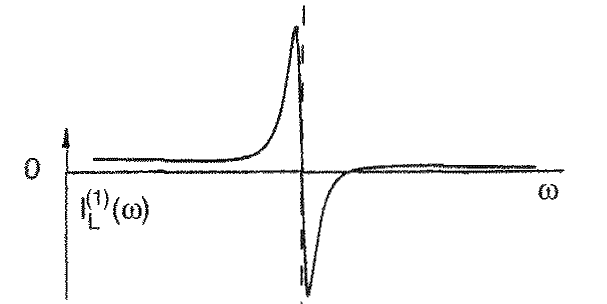
\includegraphics[width=1\linewidth]{Images/Dispersive.png}
\caption{An example of a dispersive signal used as the error signal for locking the cooling laser.~\cite{demtroder}}
\label{fig:Dispersive}
\end{figure}

\subsection{Optical Trap}
An optical trap is organised with three lasers for the three directions of space, orientated so that they have a crossing point. Each laser is then reflected back into the gas and through this central crossing point so that there are six counter-propagating beams. This provides radiation pressure in six different directions, all directed back toward the crossing point. That said, the radiation pressure should only be imposed on atoms moving away from the trap. Otherwise, the lasers would also push out atoms in the trap and along the laser beam. As a result, the lasers are all red detuned from a particular transition such that when the atoms are moving away from the trap, these lasers are blueshifted for the atoms and become resonant with the transition allowing for the absorption of the photons. That said, the resonance of the atoms with the lasers is dependent on the velocity of the atoms. Furthermore, the probability of an atom absorbing a photon is dependent on the difference between the Doppler shifted frequency of the photon and the atom's transition frequency, as show in Figure~\ref{fig:Scat}. It can be seen that more atoms moving away from the centre will be forced back than atoms moving toward the centre. That said, using only one frequency for the lasers means that many atoms moving away from the centre of the trap will still be largely transparent to the lasers due to small scattering rates. The optical trap purely achieves an ``optical molasses" in the intersection volume of the lasers, so called because atoms moving away from the centre are slowed as if moving in a viscous medium. This molasses cannot completely stop the atoms from leaving the intersection volume however, whereby they will be lost to the trapping method, nor does it provide a point that the atoms are drawn towards. As a result, using the optical trap in conjunction with a magnetic trap is a better method.
\begin{figure} [!h]
	\centering
	\insertFigure{Images/Scat.png}
	\caption{The scattering rate and thus force from radiation pressure between the differently Doppler shifted laser photons and the atoms.~\cite{Wieman}}
	\label{fig:Scat}
\end{figure}

\subsection{Magneto-optical Trap}
A magnetic field is used to introduce a position-dependent force from radiation pressure. Two coils are arranged in an anti-Helmholtz configuration (face to face but with currents in opposing directions) to produce a quadrupole magnetic field, pictured in Figure~\ref{fig:mag}. 
\begin{figure} [!h]
	\centering
	\insertFigure{Images/Mag.png}
	\caption{A quadrupole magnetic field in 2D space. The field lines become more dense further from the centre, showing the increase in magnetic field strength.~\cite{mag}}
	\label{fig:mag}
\end{figure}
This magnetic field has a strength that increases linearly from centre, which itself has zero magnetic field. This means that the Zeeman effect, which splits previously degenerate magnetic energy levels of atoms into non-degenerate states with separation proportional to magnetic field strength $\Delta E \propto m_iB$ (where $m$ is the magnetic quantum number), increasingly separates energy levels the further from the centre an atom is. The lasers can thus be red detuned from one of these transitions such that as an atom moves away from centre, the transition becomes increasingly resonant with the laser, increasing the scattering rate. As a result, the force felt by atoms moving away from the centre of the intersection volume increases with distance, such that atoms can be more effectively trapped. This also ensures that atoms in centre of the volume will be largely transparent to the cooling lasers, as there is no magnetic field. Figure~\ref{fig:Zeeman} illustrates the Zeeman effect and resulting force on the atoms on either side of the trap. 
\begin{figure} [!h]
	\centering
	\insertFigure{Images/Zeeman.png}
	\caption{The Zeeman effect on atoms on either side of the centre where the magnetic field changes sign. The transitions allowed for differently polarised light is also shown.~\cite{Wieman}}
	\label{fig:Zeeman}
\end{figure}
As the magnetic field has a different sign on either side of the centre, a certain energy level $m_i$ will not have the same energy on either side. Circularly polarised lasers therefore need to be used, where the reflection of a laser will cause the polarisation to flip from $\sigma_-$ to $\sigma_+$ for example. The counter-propagating laser beams are thus oppositely polarised meaning that they will be resonant with different transitions, one with $m=-1$ and the other with $m=+1$. This is due to the transition selection rules where a $\sigma_\pm$ polarised photon requires that $\Delta m=\pm1$ between the initial and final states of the atom.~\cite{Foot} Though the beams are resonant to different transitions, these transitions will have the same energies the same distance away from the centre, meaning that a laser with a single frequency can become increasingly resonant atoms on either side of the atom trap. The magnetic field has thus introduced a point which the atoms are drawn towards. The complete MOT set-up is given in Figure~\ref{fig:MOT2}. The centre of the magnetic field is to be aligned with the centre of the intersection volume of the lasers to achieve the best results. \\
\begin{figure} [!h]
	\centering
	\insertFigure{Images/MOT2.png}
	\caption{The MOT set-up, shown with the coils in anti-Helmholtz configuration, magnetic field, and laser beam polarisations.~\cite{Foot}}
	\label{fig:MOT2}
\end{figure}
 
\par There is a limit to the extent that a MOT can cool down atoms. The atoms must always re-emit the energy that they have absorbed from the lasers. These photon emissions are isotropic however, leading to an average recoil force on the atom of $\langle F\rangle_{\text{recoil}}=0$~N, retaining the efficiency of the optical trap method. The atoms will nevertheless be pushed around randomly by the recoil forces during each photon emission, thus meaning that the kinetic energy and consequently temperature of the atoms will not be able to be further reduced past this point. This minimum temperature is called the Doppler limit, which is generally in the $\mu K$ for an MOT. Methods such as Bose-Einstein condensation must be used to cool down atom traps further. 

\subsection{Rubidium} \label{sec:Rubidium}
Natural Rubidium gas is composed of $^{85}\ce{Rb}$ and $^{87}\ce{Rb}$. This experiment focuses on $^{85}\ce{Rb}$ as it is approximately three times more abundant in the gas. The level structure of $^{85}\ce{Rb}$ is given in Figure~\ref{fig:Spectrum}. The transition used in this experiment for resonance with the cooling lasers with $\sigma_+$ polarisation is the F=3 (or m=3) $\to$ F'=4 transition. This transition is nominally closed meaning that excited atoms can only decay down into the F=3 state. This means that are continuously able to absorb photons from the cooling lasers, allowing for further cooling and trapping. There are rare excitations to the F'=2,3 states however which can decay to the F=2 ground state which is no longer resonant to the cooling lasers. As a result, a repumping laser tuned to the F=2 $\to$ F'=3 transition is introduced to pump atoms back into states sensitive to the cooling lasers when they decay to the F=3 state. One should note that $^{87}\ce{Rb}$ is still present in the gas and that its spectrum will be visible.
\begin{figure} [!h]
	\centering
	\insertFigure{Images/Spectrum.png}
	\caption{The energy levels $^5S_{1/2}$ and $^5P_{1/2}$ of $^85\ce{Rb}$. The cooling laser and repumping laser transitions used are the F=3 $\to$ F'=4 and F=2 $\to$ F'=3 transitions respectively.~\cite{Wieman}}
	\label{fig:Spectrum}
\end{figure}

\subsection{Diode Laser} \label{sec:laser}
Diode lasers are used in this experiment for the cooling and repumping lasers. The reasons for this are that the state transitions we exploit for cooling and repumping lie in the infrared range and that we need tunable coherent light sources.Diode lasers work via the recombination of an electron with a hole in a diode, resulting in electromagnetic radiation with a large linewidth, which starts the laser oscillations.~\cite{demtroder} In the laser diode, the metal case used for heat dissipation and the optical cavity makes it possible that population inversion can occur above a threshold current, which means a large free spectral range can be lased. In order to produce a laser with a single mode instead, a grating is used as shown in Figure~\ref{fig:Diode}. Here, the laser produced by the diode is divergent and collimated to a non-divergent beam by the collimating lens.
\begin{figure} [!h]
	\centering
	\insertFigure{Images/Diode.png}
	\caption{The diode laser with the grating in Littrow configuration.\cite{manual}}
	\label{fig:Diode}
\end{figure}
The beam is then directed on to an external grating in Littrow configuration, as seen in Figure~\ref{fig:Grating}. The grating is positioned such that for the desired frequency, the $-1.$ order is reflected back into the active medium, thus serving as an external resonating element. This back-reflected frequency determines the single-mode frequency of the laser. The actual beam produced for use is the $0.$ order, which makes up most of the produced power of the laser diode. For constructive interference, the grating equation reads as given in Figure~\ref{fig:Grating}, such that a single mode is obtained.
\begin{figure} [!h]
	\centering
	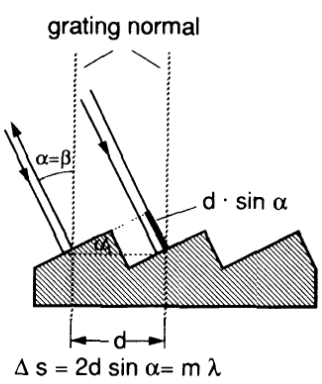
\includegraphics[scale=0.4]{Images/Grating.png}
	\caption{Diffraction grating in a Littrow configuration, when the incident and reflected beams coincide.~\cite{demtroder}}
	\label{fig:Grating}
\end{figure}
A piezo system functioning on triangular supply voltage, as well as adjustable screws, are responsible for the moving of the grating so that different frequencies in the laser spectrum can be reflected back to the laser, allowing for frequencies of the laser to be scanned. The error signal produced by polarisation spectroscopy, discussed in Section~\ref{sec:pol}, is that used as the triangular voltage to stabilise and lock the laser to a desired frequency. The frequency can also be changed with the current applied to the diode and the diode's temperature, such that changes in the temperature of the room causes the frequency of the laser to drift.

\section{Experimental Set-up} \label{sec:Exp}
The laser section of the experiment is shown in Figure~\ref{fig:Laser}.
\begin{figure} [!h]
	\centering
	\insertFigure{Images/Laser.png}
	\caption{The set-up for producing the cooling and repumping lasers, sent to the MOT experiment.~\cite{manual}}
	\label{fig:Laser}
\end{figure}
This produces both cooling and repumping lasers which are sent to the MOT set-up collinear through an optical fibre. Two cells with Rubidium gas are used for the polarisation spectroscopy to produce the error signals to scan and lock both lasers. This part of the experiment was already configured.

\subsection{MOT Set-up and Procedure}
The MOT set-up is shown in Figure~\ref{fig:MOT}.
\begin{figure} [!h]
	\centering
	\insertFigure{Images/MOT.png}
	\caption{The MOT set-up.\cite{manual}}
	\label{fig:MOT}
\end{figure}
A vacuum chamber held at pressure levels of approximately $10^{-7}$~mbar with glass windows served as the container for the Rubidium gas. The collinear cooling and repumping beams were directed by two beam splitters, several mirrors, and six quarter waveplates for each of the beams convergent on the atom trap. The six beams could be adjusted by fine-tuning the mirror angles with screws. The two coils which provided the magnetic field were fixed in space, thus providing a fixed magnetic field. The strength of the magnetic field could be altered however, by changing the current applied to the coils. Acquiring a MOT was the first aim of the experiment. To do so, the six laser beams had to be aligned such that they formed an intersection volume in the centre of the magnetic field. Markings on the vacuum cell container gave approximate indications of the centre of the magnetic field. An infrared camera was also used to see the fluorescence of the laser beams in the vacuum cell and thus the laser beams themselves. Using these two devices, the beams were aligned to cross approximately at the centre of the magnetic field. It was necessary to make sure that none of the laser beam profiles were cut so that as little power was lost. Furthermore, in order to make sure that the laser beams were reflected adequately back into the gas along the beams of the incident lasers, the mirrors were fine-tuned so that the beams were reflected back into the optical fibre. This was achieved by using a piece of paper with a small hole in it to allow the incident beam near the optical fibre to pass through and seeing on the paper how far the reflected beams were from being reflected perfectly back through the hole. The mirrors were adjusted until thus was achieved. \\
\begin{figure} [!h]
	\centering
	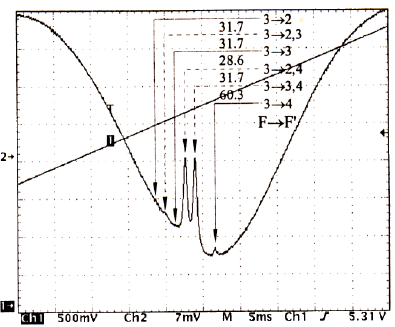
\includegraphics[width=0.95\linewidth]{Images/Peaks.png}
	\caption{$_{85}$Rb observed spectrum with Lamb dips for $F = 3 \rightarrow F' = 2, \, 3, \, 4$. The transitions to states with two numbers refer to crossover peaks.\cite{manual}}
	\label{fig:Peaks}
\end{figure}
\par Once an intersection was accomplished, the spectrum of the gas was obtained on an oscilloscope by scanning the cooling laser, as shown in Figure~\ref{fig:Peaks}. When the peak for the desired F=3 $\to$ F'=4 transition was found, the laser was locked to a frequency slightly red detuned from this as a guess. For the repumping laser, the F=2 $\to$ F'=3 transition was found in the spectrum, shown in Figure~\ref{fig:Peaks}, and the laser was made to scan a small range over the peak. The laser was not detuned as it is not used to cool the atoms, just to repump atoms lost to the cooling process. Furthermore, it was not locked for most of the experiment as it was found that a large MOT was obtained when it was made to scan a small range. This is thought to be due to the ability for the laser to be resonant with more atoms of different speeds and different positions in the magnetic field. 
\begin{figure} [!h]
	\centering
	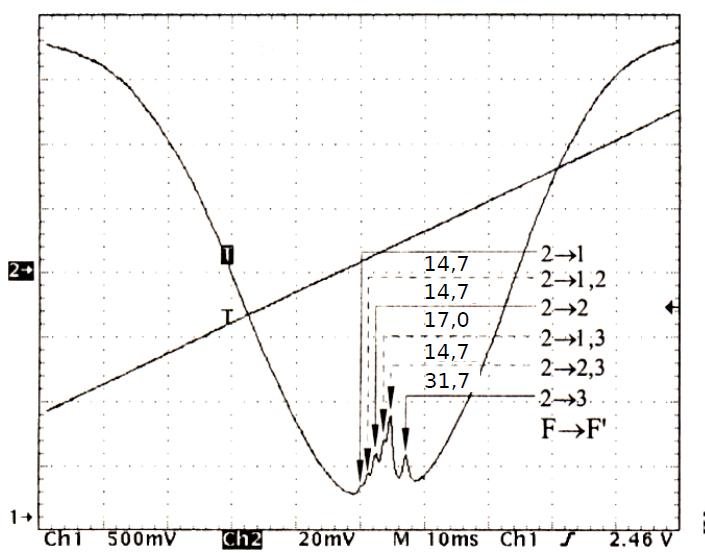
\includegraphics[width=1\linewidth]{Images/Peak1.png}
	\caption{$_{85}$Rb observed spectrum with Lamb dips for $F = 2 \rightarrow F' = 1, \, 2, \, 3$. The transitions to states with two numbers refer to crossover peaks.\cite{manual}}
	\label{fig:Peaks1}
\end{figure}
The frequencies of the lasers were then fined tuned, especially that of the cooling laser, until a MOT was observed by a video camera able to see the infrared fluorescence emitted. A ferromagnet was also used to affect the magnetic field of the coils to see whether a MOT could be observed. This would suggest that the intersection point of the laser beams were not properly aligned with the centre of the magnetic field and that they needed to be re-aligned. Once a lasting MOT was observed with adequate luminescence, the quantitative measurements were undertaken. Due to the laser drift caused by the ambient temperature change, the measurements had to be performed quickly.

\section{Results}

\subsection{Laser Beam Diameter} \label{sec:diam}
Using a movable razor blade and a powermeter, the intensity of the combined cooling and repumping laser beam as a function of the displacement of the blade along an axis perpendicular to the beam propagation, thereby blocking parts of the beam, was measured. This allowed an investigation into the profile of the laser beam. The results are collected in Table~\ref{table:beampower}. 
\begin{table} [!h]
	\centering
	\begin{tabular}{|c|c|}
		\hline
		Position (cm)	& Power (mW)\\
		\hline
		$39.4 \pm 0.05$	&	$1.58 \pm 0.08$\\ 	\hline
		$39.5 \pm 0.05$	&	$1.57 \pm 0.08$\\ 	\hline
		$39.6 \pm 0.05$	&	$1.52 \pm 0.08$\\ 	\hline
		$39.7 \pm 0.05$	&	$1.40 \pm 0.07$\\ 	\hline
		$39.8 \pm 0.05$	&	$1.07 \pm 0.05$\\ 	\hline
		$39.9 \pm 0.05$	&	$0.62 \pm 0.03$\\ 	\hline
		$40.0 \pm 0.05$	&	$0.25 \pm 0.01$\\ 	\hline
		$40.1 \pm 0.05$	&	$0.10 \pm 0.01$\\ 	\hline
		$40.2 \pm 0.05$	&	$0.04 \pm 0.01$\\	\hline
		$40.3 \pm 0.05$	&	$0.01 \pm 0.01$\\	\hline
		$40.4 \pm 0.05$	&	$0.00 \substack{+0.01 \\ -0.00}$\\	\hline
	\end{tabular}
	\caption{Beam power as a function of position of the razor blade. The last value has no negative uncertainty as the powermeter didn't read a negative value in this mode, even when it was blocked from light. The last few readings have higher uncertainty due to larger reading fluctuations observed.}
	\label{table:beampower}
\end{table}
The uncertainty in the power measurements is a result of their sensitivity to very slight movements of the blade, less than was noticeable. The errors were estimated to be approximately 5\% for all values by repeating measurements of different values and quantifying their deviation. Laser beams have Gaussian profiles thus meaning that the power of the beam should follow an error function as it is an integral of a Gaussian~\cite{beam}. Fitting such a function
\begin{alignat*}{2}\label{erf}
f(x) &= \mathrlap{P + A \cdot \text{erfc}(B\cdot x - C),}
\shortintertext{we found}
P &= (0.0066 \pm 0.0005) \, \text{mW},\\
A &=  (0.748\pm 0.016) \, \text{mW},\\
B &=  4.681 \pm 0.095,\\
C &= 187.6 \pm 3.8.
\end{alignat*}
This results in a width of the laser beam of %http://people.fjfi.cvut.cz/blazejos/public/ul7en.pdf
\begin{equation}
w = (0.2860 \pm 0.0077) \, \text{ cm}. \nonumber
\end{equation}
The results with the fit are plotted in Figure~\ref{fig:beam}, showing good agreement between the measurements and the fit.
\begin{figure} [!h]
	\centering
	\insertFigure{Images/beam.png}
	\caption{Plot of the laser beam luminosity with razor blade position, provided with fit.}
	\label{fig:beam}
\end{figure}

\subsection{Size of the MOT}
To get an estimate of the MOT size, we took a photo of it from the side, shown in Figure~\ref{fig:mot_w_scale}. The photo is superimposed with a photo of a ruler placed the same distance away from the camera as the MOT. This was achieved by moving the ruler back and forth until it was in the focus of the camera and was done so that a scale for the MOT image could be used to convert distances in pixels to centimetres.
\begin{figure} [!h]
	\centering
	\insertFigure{Images/MOT_w_scale_crop.png}
	\caption{Photo of the MOT merged with photo of the scale.}
	\label{fig:mot_w_scale}
\end{figure}
The MOT as well as the vertical and horizontal laser beams can be seen in the photo. An image software determined that two points $\SI[separate-uncertainty = true]{30.0 \pm 0.5 }{\milli\meter}$ away from each other in the image were separated by $742.2$ pixels. The uncertainty here is due to the width of the millimetre lines on the scale and the two points not at the same distance from the edge of the ruler. Thus
\begin{equation}
1 \text{~px} = \SI[separate-uncertainty = true]{40.42 \pm 0.67}{\micro\meter}. \nonumber
\end{equation}
As visible in Figure~\ref{fig:mot_w_scale}, the MOT does not have a perfect circular cross-section. This is likely the result of the laser beams not intersecting to form a perfect cubic intersection volume and not being exactly centred with the magnetic field. The latter can be directly observed in the photo from the discrepancy between the position of MOT and the centre of the intersection of the beams. The directly measured width and height for the MOT are
$$
h = (72 \pm 2)  \, \text{px}, \: \text{and} \: w = (57 \pm 2)  \, \text{px}.
$$
We chose to approximate the volume by an ellipsoid with one axis half the height ($c$) and two axes half the width ($a$, $b$) each, as our best guess is that the MOT is just as deep as it is wide. That said, the imaged cross-section of the MOT is nearly circular thereby giving more some assurance that the real depth wasn't too different from our estimation. The dimensions of the MOT and its volume were calculated to be
\begin{align*}
a, b &= \SI[separate-uncertainty = true]{1.15 \pm 0.04}{\milli\meter}, \\
c &=  \SI[separate-uncertainty = true]{1.46 \pm 0.05}{\milli\meter}, \\
V &= \frac{4}{3} \pi a b c = \SI[separate-uncertainty = true]{8.09 \pm 0.52 }{\cubic\milli\meter}.
\end{align*}

\subsection{Magnetic Field Dependence}
To measure the MOT fluorescence as a function of the magnetic field, we changed the current flowing through the coils. The luminosity of the fluorescence was measured with a powermeter directed at the MOT. Figure~\ref{fig:magnetic} shows our results. 
\begin{figure} [!h]
	\centering
	\insertFigure{Images/magnetic_dependence_w_linear.png}
	\caption{The dependency of MOT luminosity on the current flow through the coils and thus the strength of the magnetic field, given with linear fit.}
	\label{fig:magnetic}
\end{figure}
The plot seems to suggest that the MOT luminosity follows a sigmoid curve relationship with magnetic field strength, though it is nearly linear. To get a visible MOT, we had to set the current to a minimal value of around $0.9$~A. From this point, it can be seen that the fluorescence grew approximately proportional to the current, up to $4.6$~A. The background fluorescence from the lasers and the environment was previously measured and subtracted from the data. A linear fit was performed for the central linear section, with calculated coefficients $a = 22.11 \pm 0.53$~nW/A and $\text{const} = -20.9 \pm 1.5$~nW. It can be seen that the full plot is not linear. Further experiments can aim at obtaining a more luminous MOT in order to determine whether this relationship is indeed linear or sigmoid-like, or neither.

\subsection{Influence of Quarter Waveplates}
The influence of the quarter waveplate angles were then measured. Firstly, the angle of the quarter waveplate for one of the beams before it first passes through the vacuum cell was scanned. This is illustrated as one of the two quarter waveplates on the lower half of Figure~\ref{fig:MOT}. Changing this quarter plate thus also affects the polarisation of the reflected beam, given that the relative angle between the two waveplate changes. The powermeter was again used to measure the MOT luminosity. The background luminosity was subtracted from the data and a plot of the results with a periodic fit is given in Figure~\ref{fig:Waveplate}. The function of the fit is
\begin{equation}
f(x) = A \cos\big(x - \varphi \big) + B, \nonumber
\end{equation}
which produced coefficients
\begin{align*}
A &=  (74.9 \pm 5.4) \, \text{nW},\\
B &=  (9.8 \pm 3.3) \, \text{nW},\\
\varphi &=  (404.66 \pm 2.1)^\circ.
\end{align*}
A periodic fit is expected as this changes the circular polarisation of the cooling beams and thus they become less or more detuned with the cooling transition, hence affecting the efficacy of trapping the atoms. It is expected that there be minima at $\theta=90^\circ, 180^\circ$ and maxima at $\theta=0^\circ, 90^\circ$ as this is when the beams become perfectly circularly polarised or stay completely linearly polarised, respectively. 
\begin{figure} [!h]
	\centering
	\insertFigure{Images/Waveplate1_w_fit.png}
	\caption{MOT luminescence intensity as a function of the polarization angle of the first quart waveplate.}
	\label{fig:Waveplate}
\end{figure}
The results show a shift from this expectation. This is expected to be as a result of the laser light being linearly polarised with $\theta=140^\circ$ or $320^\circ$ with respect to the quarter waveplate, as opposed to $0^\circ$. Further experimentation can investigate this reasoning. Regardless, a periodic relationship has been found as expected. The measurements do not fit the function very accurately however, resulting from a larger number of measurements at lower luminosity near the minima. This could be due to the MOT's higher sensitivity to the proper detuning of the laser, as was observed, thus suggesting that the relationship is indeed not perfectly sinusoidal. Further experiments should aim to obtain more precise data with a more stable MOT to determine relationship more accurately. \\

\par The angle of the second quarter waveplate after the beam was reflected back into the vacuum cell was then scanned. Changing this waveplate does not affect the polarisation of the incident beam obviously, thus serving as a different investigation to the one above. The results are displayed in Figure~\ref{fig:Waveplate2}.
\begin{figure} [!h]
	\centering
	\insertFigure{Images/Waveplate2.png}
	\caption{MOT luminescence intensity as a function of the polarization angle of the second quarter waveplate, given with a fit.}
	\label{fig:Waveplate2}
\end{figure}
The underlying relationship foremostly appears to be a constant function, shown as the red dashed fitted line. This is to be expected as the beam actually passes through this quarter waveplate twice, once incident on the mirror and then a second time after it has been reflected, as can be seen in Figure~\ref{fig:MOT}. Passing twice through this quarter waveplate is equal to passing once through a half waveplate, thus changing the orientation of linearly or circularly polarised light. As the first quarter waveplate was set so that the beam was circularly polarised, passing through the second quarter waveplate will simply convert $\sigma_\pm$ polarisation to $\sigma_\mp$, irrespective of the angle of the quarter waveplate. Thus, a constant MOT luminosity is expected, as was observed. The large uncertainties and deviations from a constant value are largely a cause of the fluctuations seen in the luminosity values due to the sensitivity of the entire experiment.

\subsection{Loading Time and Cross-section}
The characteristic loading time of the obtained MOT was observed next, measured using a photodiode instead of the powermeter and displaying its signal on an oscilloscope. The repumping laser was also locked when using the photodiode as the photodiode was sensitive to slight luminosity fluctuations that the powermeter was blind to. The loading time was obtained by turning off the magnetic field so that no MOT was observed and then turning it back on with its maximum value and observing the luminosity of the MOT as a function of time. Data was obtained for six separate MOT loading events to find the characteristic loading time. Figure~\ref{fig:buildup} shows one such event with a fit. 
\begin{figure} [!h]
	\centering
	\insertFigure{Images/mot_buildup.png}
	\caption{Example of data points exported from the oscilloscope with the fitted function in red. The measurements and the fit were in good agreement for all six events.}
	\label{fig:buildup}
\end{figure}
It is known that the number of trapped atoms changes as~\cite{Wieman} 
\begin{equation}\label{eq:load}
N(t) = N_0 \big( 1 - e^{-\frac{t}{\tau}} \big),
\end{equation}
where $\tau$ is the loading time and $N_0$ is the maximal number of atoms in the trap. This is the function that was used for the fit in Figure~\ref{fig:buildup}. The scattering cross-section $\sigma$ of the atoms is related to $\tau$ if there is only $\ce{Rb}$ in the vacuum chamber, which is a valid approximation given the high vacuum achieved in the cell. The cross-section is related by
\begin{equation}\label{eq:cross-section}
\frac{1}{\tau} = n \sigma v, \nonumber
\end{equation}
where $n$ is the number density and $v$ is the average velocity of the $\ce{Rb}$ gas. This will allow for a calculation of the cross-section of the Rubidium gas. As the luminosity against time signal measured also follows Equation~\ref{eq:load}, by fitting such a function to the oscilloscope data and averaging across the six different events, we calculated a loading time of 
\begin{equation}
\tau = (0.268 \pm 0.006) \, \text{s}.\nonumber
\end{equation}
With the recorded temperature $T = (293.55 \pm 0.05) \, K$ of the room and the pressure $p = (8.09 \pm 0.01)\cdot 10^{-8} \, \text{mbar}$ of the vacuum cell, as well as the mass of $^{85}\ce{Rb}$ being $m = 141.037 \times 10^{-27} \, \text{kg}$, the average velocity of the gas was calculated as
%mass of 85 Rb: 84.911 amu = 141.037*10^-27 kg
\begin{equation}
v = \sqrt{\frac{2kT}{m}} = (293.545 \pm 0.025) \, \frac{\text{m}}{\text{s}}, \nonumber
\end{equation}
and the number density $n$ was calculated from the ideal gas law as
\begin{equation}
n = \frac{N}{V} = \frac{p}{kT} = (1.9970 \pm 0.0025)\cdot 10^{15} \, \frac{1}{\text{m}^3}.\nonumber
\end{equation}
Thus, the cross-section of the gas was calculated to be
\begin{equation}
\sigma = \frac{1}{n \tau v} = (6.36 \pm 0.13) \cdot 10^{-18} \, \text{m}^2. \nonumber
\end{equation}
This is in agreement with previous experimentation~\cite{cross} giving confidence to our method and results.

\subsection{Influence of Laser Detuning} \label{sec:det}
The influence of the frequencies of both the cooling and repumping lasers on the luminosity and thus size of the MOT were then observed. Both the photodiode and spectrum signal used to lock the laser were connected to an oscilloscope so that both the spectrum and fluorescence signal were displayed together. The laser was then made to scan a range of frequencies on its spectrum near the transition of interest for the respective laser. The scan was set to 50~mHz so that the laser the frequencies slower than the loading time of the MOT, allowing for a MOT to become populated if possible at a certain frequency. Figure~\ref{fig:Detuning} is a plot of the cooling laser spectrum scanned with respective MOT fluorescence for those frequencies. The repumping laser was left locked at its optimal point.
\begin{figure} [!h]
	\centering
	\insertFigure{Images/Detuning1.png}
	\caption{MOT luminescence (red) and cooling laser frequency (blue) plotted against time during the scan, with the signal amplitudes adjusted so that they could be plotted in the same window with a high level of detail. The data was exported from the oscilloscope. Known Lamb dips and crossover peaks in the spectrum are labelled, as well as the peak in luminescence when a MOT was observed. Peaks 1, 2, and 3 are the F=3 $\to$ F'=2,4 crossover peak, F'=3,4 crossover peak, and F'=4 Lamb dip.}
	\label{fig:Detuning}
\end{figure} 
The spectrum in blue obtained in the figure is in good agreement with that expected from Figure~\ref{fig:Peaks}. Furthermore, the peak MOT fluorescence is seen as a sharp peak slightly redshifted from the F=3 $\to$ F'=4 transition, as expected. The known frequencies of the Lamb dips and crossover peaks found allows for a scaling between the time of the scan and the frequency being scanned at that time. From this scale, the frequency of the cooling laser at which the most luminescent MOT was obtained can be calculated, allowing for a precise calculation of the ideal red detuning for the cooling laser. The detected peaks and the maximum MOT fluorescence observed are measured at
\begin{alignat*}{3}
&F=3 \rightarrow F'=2, \, 4&&: \hspace{12pt} &(4.708 \pm 0.024) \, \text{s},\\
&F=3 \rightarrow F'=3, \, 4&&:  &(4.956 \pm 0.024) \, \text{s},\\
&F=3 \rightarrow F'=4&&:		 &(5.556 \pm 0.016)\, \text{s},\\
&MOT			&&:		&(5.456 \pm 0.008) \, \text{s}.
\end{alignat*}
The uncertainty in these values are determined by quantifying the range of values which would still be reasonable for the position of the respective peak, with the centre proving as the used value for the peak position. By matching the difference of peaks 1 and 2, and peaks 2 and 3 with the differences in the frequencies of these transitions, and then averaging the results, yields a frequency-time scale of
\begin{equation}
C =(114 \pm 11)\, \frac{\text{MHz}}{\text{s}}. \nonumber
\end{equation}
The optimal detuning then is the difference between the MOT fluorescence peak and the F=3 $\rightarrow$ F'=4 peak:
\begin{equation}\label{eqn:detuning}
\Delta \nu = C \cdot (0.100 \pm 0.008) \, \text{s} = (11.4 \pm 1.4) \, \text{MHz}.
\end{equation}
This is in agreement with the spectrum of $^{85}\ce{Rb}$ and the optimal locking place found for the cooling laser. \\

\par The process was then repeated for the repumping laser, leaving the cooling laser locked on the optimal frequency. The plotted results are given in Figure~\ref{fig:det} with a double Gaussian fit of the two spectrum peaks.
\begin{figure} [!h]
	\centering
	\insertFigure{Images/Detuning2.png}
	\caption{MOT luminescence (red) and repumping laser frequency (blue) plotted against time during the scan. A double Gaussian fit of both spectrum peaks is plotted in black and the estimated position of the MOT luminescence peak is given by the dotted line. By comparison to the known spectrum, the spectrum peaks are identified as the F=2 $\to$ F'=2,3 crossover peak and the F'=3 Lamb dip from left to right.}
	\label{fig:det}
\end{figure}
Here, the peak in MOT luminosity is far more spread out than when scanning the cooling laser. This is what was observed during the previous experiments and the reason why locking the repumping laser was not necessary, instead letting it scan over a small frequency range over the bump. That said, the resolution of the peak is poor, possibility hiding more detail in the frequency-dependent MOT luminosity in this bump. There shouldn't be reason to doubt the measured maximum in luminosity however, which is the most important detail. Furthermore, the peak is indeed found slightly red detuned from the used F=2 $\to$ F'=3 transition, as expected. The position of the spectrum peaks were calculated using the Gaussian fits while the position of the fluorescence peak was determined manually as for the cooling laser peaks. Their positions are
\begin{alignat*}{3}
&F = 2 \rightarrow F'=2, \, 3&&: \hspace{12pt} &(2.2520 \pm 0.0033) \, \text{s},\\
&F=2 \rightarrow F'=3 &&:  &(4.0136 \pm 0.0043) \, \text{s},\\
&MOT			&&:		&(3.71 \pm 0.05) \, \text{s}.
\end{alignat*}
Using the same method as above, the MOT peak was calculated to be red detuned from the F=2 $\to$ F'=3 peak by $\Delta \nu = (5.53 \pm 0.90)\, \text{MHz}$. The position of the bump with respect to the spectrum is indeed in agreement with where the repumping laser was allowed to scan and at times locked in order to obtain a MOT.

\subsection{MOT Population}
Using the MOT fluorescence, the total radiative power of the MOT, the detuning of the cooling laser determined in Section~\ref{sec:det}, and the beam power and diameter determined in Section~\ref{sec:diam}, the total number of Rubidium atoms in the MOT can be determined. The total power of the laser beam was measured as $P = 10.60 \pm 0.05$~mW giving a total intensity of beam of
\begin{equation}
I = \frac{2 P}{\pi w^2} = (73.9 \pm 3.0) \frac{\text{mW}}{\text{cm}^2}. \nonumber
\end{equation}
This can then be used to calculate the photon scattering rate $R$ with the Rubidium, given by the following equation~\cite{Wieman}:
\begin{equation}
R = \frac{\Gamma}{2} \frac{\frac{I}{I_{\text{sat}}}}{1 + \frac{I}{I_{\text{sat}}} + \left( \frac{2 \Delta \nu}{\Gamma} \right)^2} = (18.492 \pm 0.043)\, \text{MHz,} \nonumber
\end{equation}
where $\Gamma = 2 \pi \cdot (6.0666 \pm 0.0018)$~MHz is the natural linewidth of the transition~\cite{steck}, $I_{\text{sat}} = (1.66932 \pm 0.00035)\, \frac{\text{mW}}{\text{cm}^2}$ is the saturation intensity~\cite{steck}, and $\Delta \nu$ is the detuning of the cooling laser calculated by Equation~\ref{eqn:detuning}. \\

\par The total intercepted power at a distance $\rho$ from the MOT by a lens with radius $r$, when the MOT has a radiation power $P_{\text{MOT}}$, is 
\begin{equation}
P = \frac{P_{\text{MOT}}}{4 \pi \rho^2} \cdot \pi r^2, \nonumber
\end{equation}
where we measured $\rho = (10.5 \pm 1.0) \,$cm and $2r = (2.5\pm 0.1) \,$cm. Thus, the MOT's radiative power was
\begin{equation}
P_{\text{MOT}} = 47.4 \pm 9.8 \, \text{$\mu$W}. \nonumber
\end{equation}
The large error in this value is mainly due to the large uncertainty in the distance measurement which was difficult to determine as a result of the vacuum cell being in the way and because the exact location of the invisible MOT was unknown. The total number of trapped atoms can now be calculated using the following relation~\cite{Wieman}:
\begin{equation}
P_{\text{MOT}} = N R h \nu, \nonumber
\end{equation}
where $\nu$ is the locked frequency of the cooling laser. This gives a population size of
\begin{equation}
N = (10.1 \pm 2.1)\cdot 10^6. \nonumber
\end{equation}
This is in good agreement with literature on this experiment~\cite{Wieman}, who trapped approximately four times more atoms. Indeed, we found that we could not obtain an MOT with as high luminosity as was achieved in similar experiments~\cite{manual} due to time constraints. Ultimately, the previous calculations aimed at characterising the obtained MOT could have been improved by obtaining a larger and more stable MOT.

\section{Conclusion}
We setup an experiment to obtain a MOT, optimised it, and then took measurements to characterise it. We first measured the beam profile of the combined cooling and repumping laser beam using a razor blade and calculated its diameter as $(0.2860 \pm 0.0077) \, \text{cm}$. Next we estimated the size of the obtained MOT by taking a photo of it, calculating a volume of $\SI[separate-uncertainty = true]{8.09 \pm 0.52 }{\cubic\milli\meter}$. The dependence of the size of the MOT with the strength of the magnetic field was then measured to follow a linear or sigmoid curve, though further experiments should attempt to obtain a more luminous MOT such that the proper relationship can be determined. Next the effect of the quart waveplate angles for one of the laser beams was measured. It was found that the MOT luminescence follows a periodic relationship with the first quarter waveplate angle though it is not affect by the angle of the second quarter waveplate, which are both as expected. The loading time was then calculated to be $(0.268 \pm 0.006) \, \text{s}$ by measuring the loading behaviour of the MOT after the magnetic field was suddenly turned on. From this, the cross-section of the Rubidium gas was calculated as $(6.36 \pm 0.13) \cdot 10^{-18} \, \text{m}^2$ which is in agreement with previous experimentation.\\

\par Most importantly, the dependence of the MOT luminescence with the cooling and repumping lasers was measured by slowly scanning the frequencies of the lasers and measuring the MOT fluorescence at the same time. From this, the optimal red detuning of the two lasers were calculated as $(11.4 \pm 1.4) \, \text{MHz}$ from the F=3 $\to$ F'=4 transition and $(5.53 \pm 0.90)\, \text{MHz}$ from the F=2 $\to$ F'=3 transition, respectively, both in good agreement with the optimised detunings found during the experiment. The detuning of the cooling laser finally allowed for a calculation of the population of MOT of $(10.1 \pm 2.1)\cdot 10^6$ atoms, which is in good agreement with past experiments. Though the results obtained are largely what was to be expected from past experiments and theory, more precise results could have been obtained from obtaining a more luminous and stable MOT and should thus be the aim of later experiments.

%TODO order of appearance! and reference the error function for the laser profile
\begin{thebibliography}{9}
\bibitem{manual}
Unspecified Author, \textsl{Advanced Lab Course Experiment: Rubidium MOT} (University of Bonn, 2017).
\bibitem{demtroder}
W. Demtröder, \textsl{Laser Spectroscopy, Basic Concepts and Instrumentation} (Springer, Berlin, 2003).%Third Edition
\bibitem{Wieman}
C. Wieman and G. Flowers, American Journal of Physics 63 (1995), pp.317-30.
\bibitem{mag}
A. Wolski, \textsl{Maxwell's equations for magnets} (University of Liverpool, 2014), \url{https://arxiv.org/pdf/1103.0713.pdf}.
\bibitem{Foot}
C. J. Foot, \textsl{Atomic Physics} (Oxford University Press, New York, 2005).
\bibitem{beam}
W, Boyd, \textsl{Nonlinear Optics}, Third Edition (Academic Press, Oxford, 2008).
\bibitem{cross}
D. Fagnan, B.Sc. thesis, The University of British Columbia, 2009.
\bibitem{steck}
D. A. Steck, \textsl{Rubidium 85 D Line Data}, \url{http://steck.us/alkalidata/rubidium85numbers.pdf}.

%not referenced
%\bibitem{laserdiode}
%\textsl{Physics Fundamentals: Laser Diode Characteristics}, %\url{https://www.sukhamburg.com/download/fundamentals-laserdiodes.pdf}.



\iffalse
%Leaving this here as examples for referencing different media
\bibitem{book}
K. Siegbahn, \textsl{Alpha-, beta-, and gamma-ray spectroscopy, Vol. 2} (North Holland Publishing Company, Amsterdam, 1965).
\bibitem{booklet}
Unspecified author, \textsl{Advanced Laboratory Course (physics601): Description of Experiments} (University of Bonn, 2018).
 \bibitem{link}
 W. U. Boeglin, \textit{Scintillation Detectors}, WWW Document, \url{http://wanda.fiu.edu/teaching/courses/Modern_lab_manual/scintillator.html}.
\bibitem{pdf_on_website}
Unspecified author, \textsl{Gamma Ray Spectroscopy} (University of Florida, 2013), \url{https://www.phys.ufl.edu/courses/phy4803L/group_I/gamma_spec/gamspec.pdf}.
\bibitem{journal}
E. Ermis and C. Celiktas, International Journal Of Instrumentation Science 1, (2013), pp.54-62.
%alternative url: https://en.wikipedia.org/wiki/Constant_fraction_discriminator
\bibitem{}
M. Nakhostin, \textsl{Signal Processing for Radiation Detectors} (John Wiley $\&$ Sons, 2018), p. 298\footnote{Relevant pages (chapter 6) available for preview under\\ \url{https://books.google.de/books?id=Lrg4DwAAQBAJ}}.
%Mohammad Nakhostin
\bibitem{}
W. R. Leo, \textsl{Techniques for Nuclear and Particle Physics Experiments} (Springer-Verlag, 1987), p. 305.
%William R. Leo
\bibitem{}
A. C. Melissinos, J. Napolitano, \textsl{Experiments in Modern Physics, 2\textsuperscript{nd} edition} (Academic Press, San Diego, 2003), pp 419-21.
\fi
\end{thebibliography}
\end{document}